\chapter{Achtergrondinformatie}
\label{hoofdstuk:achtergrond}

Vooraleer we ons eigen onderzoek bespreken, moeten we even bepaalde achtergrondinformatie aanhalen. In dit hoofdstuk zullen we het kort hebben over onder meer \textit{lossless} en \textit{lossy} compressie, tensoren, de singulierewaardenontbinding en de Tucker-decompositie. Ten slotte doen we nog een bondige literatuurstudie.

\section{Compressie}

\subsection{Lossless compressie}

Wanneer data gecomprimeerd wordt, gebeurt dit vaak \textit{lossless}, waarbij de benodigde geheugenopslag verlaagd wordt terwijl de originele data nog steeds perfect reconstrueerbaar is. Denk bijvoorbeeld aan een zip-archief \cite{ref:zip}, waarbij \'e\'en enkele foute byte in de gedecomprimeerde data ertoe zou kunnen leiden dat een bestand onleesbaar wordt. Een ander voorbeeld van lossless compressie is het veel-gebruikte PNG-formaat \cite{ref:png} voor het opslaan van afbeeldingen. Beide maken gebruik van het onderliggende Deflate-algoritme \cite{ref:deflate}, dat we later ook zelf zullen gebruiken voor het lossless comprimeren van sequenties bytes.

\subsection{Lossy compressie}

Men kan meestal data echter veel verder comprimeren als men een zekere fout op het gedecomprimeerde resultaat tolereert. Dit noemen we \textit{lossy} compressie. Een typisch voorbeeld hiervan is het bekende JPEG-compressie-algoritme \cite{ref:jpeg} voor afbeeldingen. Aangezien we bij het opslaan van hyperspectrale afbeeldingen zelden ge\"interesseerd zijn in perfecte reconstructies, zullen we ons in deze thesis beperken tot het onderzoeken van lossy compressie van hyperspectrale afbeeldingen.

\newpage
\section{Multilineaire algebra}

\subsection{Tensoren}

In de lineaire algebra zijn we vertrouwd met vectoren en matrices. Er bestaat echter een veralgemening van dit concept: de tensor. Vanuit een informatica-standpunt is een tensor simpelweg een \textit{array} met een arbitrair aantal dimensies. Zo is een vector een 1D-tensor en een matrix een 2D-tensor. We zullen het aantal dimensies van een tensor vanaf nu meestal het aantal modes noemen, dit vermijdt namelijk verwarring met bijvoorbeeld de dimensie van ruimtes opgespannen door vectoren uit de tensor. De hyperspectrale afbeeldingen die we gaan comprimeren zullen we dus voorstellen als 3D-tensoren, met twee spatiale modes en \'e\'en spectrale mode.

\subsection{Vezels, matricisaties en mode-n product}

Men kan uit een tensor een reeks vectoren halen volgens een bepaalde mode. We noemen dit de mode-k vezels van de tensor \cite{ref:kolda}. Formeel komt dit voor een tensor $X$ met $d$ modes en vorm $n_1 \times n_2 \times \dots \times n_d$ neer op de verzameling vectoren:
\[
\left\{
\quad
\left.
\begin{bmatrix}
x_{i_1, \dots, i_{k-1}, 1, i_{k+1}, \dots, i_d} \\
x_{i_1, \dots, i_{k-1}, 2, i_{k+1}, \dots, i_d} \\
\dots \\
x_{i_1, \dots, i_{k-1}, n_k, i_{k+1}, \dots, i_d}
\end{bmatrix}
\quad
\right\vert
\quad
\forall i_1, \dots, i_{k-1}, i_{k+1}, i_d
\quad
\right\}
\]
Dit concept wordt gevisualiseerd in figuur \ref{fig:fibers} aan de hand van een 3D-voorbeeld.

\begin{figure}[H]
  \centering
  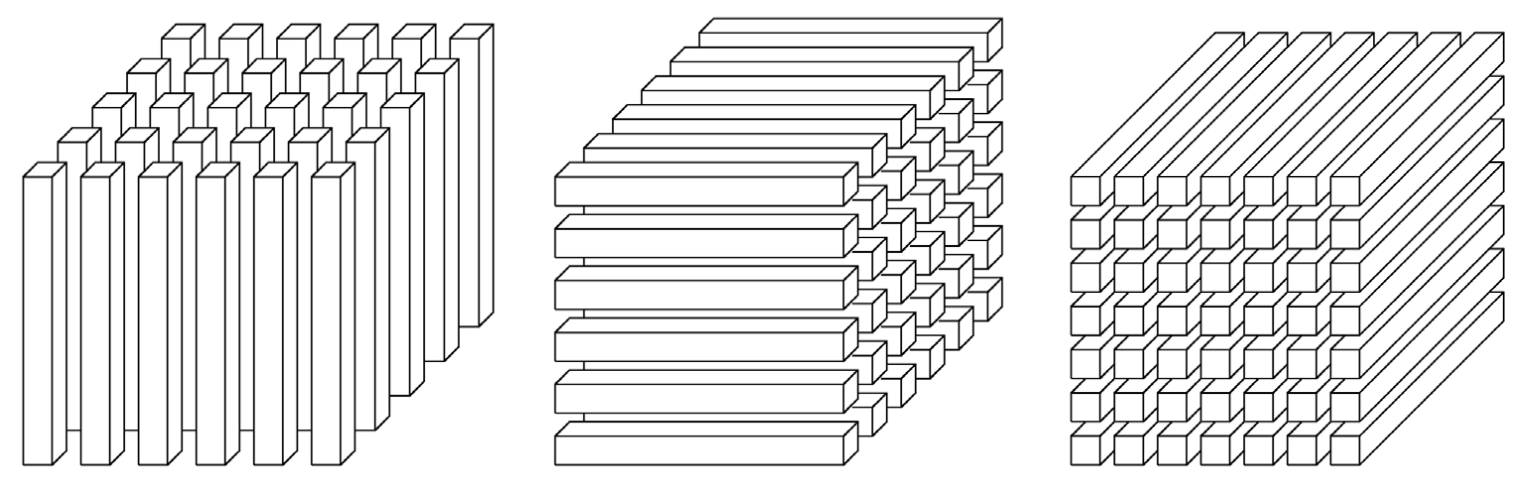
\includegraphics[scale=0.2]{images/fibers.png}
  \caption{De mode-1, mode-2 en mode-3 vezels van een 3D-tensor. Bron: Kolda en Bader \cite{ref:kolda}.}
\label{fig:fibers}
\end{figure}

Als men de mode-n vezels terug samen zet als een reeks kolommen in een matrix, bekomt men de mode-n \textit{matricisatie} van de tensor \cite{ref:kolda}. De volgorde waarin de vectoren in de matrix geordend worden, is niet van belang, zolang ze consistent is. We zullen dit opnieuw illustreren met een voorbeeld, gebaseerd op Kolda en Bader \cite{ref:kolda}. Stel we hebben een 3D-tensor $X \in \mathbb{R}^{4 \times 3 \times 2}$ waarvan de twee ``lagen'' (nu $X_1$ en $X_2$ genoemd), bepaald door de derde index, de volgende waarden bevatten:
\[
X_1 = \begin{bmatrix}
1 & 5 & 9 \\
2 & 6 & 10 \\
3 & 7 & 11 \\
4 & 8 & 12 \\
\end{bmatrix}
\quad
X_2 = \begin{bmatrix}
13 & 17 & 21 \\
14 & 18 & 22 \\
15 & 19 & 23 \\
16 & 20 & 24 \\
\end{bmatrix}
\]
\newpage
Dan zijn de verschillende mode-n matricisaties $X_{(n)}$:
\[
X_{(1)} = \begin{bmatrix}
1 & 5 & 9  & 13 & 17 & 21 \\
2 & 6 & 10 & 14 & 18 & 22 \\
3 & 7 & 11 & 15 & 19 & 23 \\
4 & 8 & 12 & 16 & 20 & 24 \\
\end{bmatrix}
\quad
X_{(2)} = \begin{bmatrix}
1 & 2  & 3  & 4  & 13 & 14 & 15 & 16 \\
5 & 6  & 7  & 8  & 17 & 18 & 19 & 20 \\
9 & 10 & 11 & 12 & 21 & 22 & 23 & 24 \\
\end{bmatrix}
\]
\[
X_{(3)} = \begin{bmatrix}
1  & 2  & 3  & 4  & 5  & 6  & 7  & 8  & 9  & 10 & 11 & 12 \\
13 & 14 & 15 & 16 & 17 & 18 & 19 & 20 & 21 & 22 & 23 & 24 \\
\end{bmatrix}
\]

Nu kunnen we ten slotte het tensor-matrix mode-n product defini\"eren. Wanneer men het mode-n product neemt van een tensor $X$ en een matrix $U$ (genoteerd als $X \times_n U$), komt dit simpelweg neer op het transformeren van alle mode-n vezels van $X$ door ze langs links te vermenigvuldigen met $U$. Formeel uitgedrukt, in functie van matricisaties en het matrix-product:
\[
Y = X \times_n U \Leftrightarrow Y_{(n)} = U X_{(n)}
\]
We zullen deze operatie zowel gebruiken om de Tucker-decompositie (later in dit hoofdstuk) en de tensor-train-decompositie (hoofdstuk \ref{hoofdstuk:hervorming}) te beschrijven.

\subsection{Singulierewaardenontbinding}

Een belangrijke matrixontbinding uit de lineaire algebra is de singulierewaardenontbinding, ook bekend als de SVD (\textit{singular value decomposition}) \cite{ref:svd}. Hierbij schrijven we de matrix $A \in \mathbb{R}^{m \times n}$ uit als het product $A = U \Sigma V^T$ waarbij $U \in \mathbb{R}^{m \times m}$ en $V \in \mathbb{R}^{n \times n}$ orthogonale matrices zijn en $\Sigma \in \mathbb{R}^{m \times n}$ een positieve diagonaalmatrix is. De kolommen van $U$ en $V$ noemen we respectievelijk de linker- en rechter-singuliere vectoren van $A$ en de diagonaalelementen van $\Sigma$ vormen de singuliere waarden van $A$ (deze staan ook gerangschikt van groot naar klein op de diagonaal).\\

Wanneer men alleen de eerste $k$ kolommen van $U$ en $V$ en de eerste $k$ diagonaalelementen van $\Sigma$ beschouwt, bekomt men de afgeknotte SVD $A_k = U_k \Sigma_k V_k^T$. Een interessante eigenschap hiervan is dat $A_k$ de beste rang-k benadering is van $A$ op vlak van Frobenius-norm. Men kan dit ook op een andere manier interpreteren: als de kolommen van $A$ een verzameling vectoren voorstellen, vormen de eerste $k$ linker-singuliere vectoren de beste $k$-dimensionale basis voor deze vectoren. Namelijk, als men de originele vectoren benadert door ze te orthogonaal projecteren op deze deelruimte, is de som van de kwadraten van de fouten op elke vector minimaal. Als men de rijen van de matrix als vectoren beschouwt, geldt hetzelfde maar dan voor de rechter-singuliere vectoren.

\subsection{Tucker-decompositie}

Een belangrijke decompositie voor tensoren is de Tucker-decompositie \cite{ref:tucker}. Hierbij wordt een tensor $A \in \mathbb{R}^{n_1 \times n_2 \times \dots \times n_d}$ met $d$ modes voorgesteld door een kerntensor $B \in \mathbb{R}^{r_1 \times r_2 \times \dots \times r_d}$ en $d$ factormatrices $U_1 \in \mathbb{R}^{n_1 \times r_1}$, $U_2 \in \mathbb{R}^{n_2 \times r_2}$, $\dots$, $U_d \in \mathbb{R}^{n_d \times r_d}$. Het verband tussen de originele tensor en de decompositie kan simpelweg gedefinieerd worden aan de hand van het mode-n product:
\[
A = B \times_1 U_1 \times_2 U_2 \times_3 \dots \times_d U_d
\]
We noemen $(r_1, \dots, r_d)$ de multilineaire rang van $B$ (later meestal de compressierang genoemd) en bijgevolg ook $A$. Stel dat we een tensor $A$ hebben met \'e\'en of meerdere modes $i$ waarvoor geldt $\text{rank}(A_{(i)}) > r_i$, dan kunnen we nog steeds een Tucker-decompositie gebruiken om $A$ benaderend voor te stellen met een (hopelijk kleine) fout, zoals we bij matrices deden met de afgeknotte SVD. Op deze manier kan men tensoren met een arbitrair aantal modes lossy comprimeren.\\

In tegenstelling tot bij matrices, is er helaas geen gekend algoritme om voor een bepaalde tensor $A$ en compressierang $(r_1, \dots, r_d)$ de optimale factormatrices $U_1, \dots, U_d$ te berekenen (als men het verschil op vlak van Frobeniusnorm probeert te minimaliseren). Er bestaat wel een iteratief algoritme, genaamd HOOI \cite{ref:kolda}, dat een lokaal optimum berekent, maar dit is te traag voor praktische doeleinden en is vooral nuttig als referentie bij het onderzoeken van de effici\"entie van niet-iteratieve algoritmen.

\subsection{T-HOSVD}

Vanwege de effectiviteit van de afgeknotte SVD bij het comprimeren van matrices, is het logisch om deze ook proberen te gebruiken voor hoger-dimensionale tensoren. Dit is wat men doet bij de T-HOSVD-procedure \cite{ref:kolda}: voor elke mode $i$ nemen we de eerste $r_i$ linker-singuliere vectoren van $A_{(i)}$ als factormatrix $U_i$. Daarna berekenen we de kerntensor $B$ door de vezels van $A$ langs elke mode orthogonaal te projecteren op de deelruimte bepaald door de corresponderende factormatrix:
\[
B = A \times_1 U_1^T \times_2 U_2^T \times_3 \dots \times_d U_d^T
\]

\subsection{ST-HOSVD}

Een andere manier om een Tucker-decompositie van een tensor te berekenen, ook gebaseerd op de SVD, is met de ST-HOSVD \cite{ref:st_hosvd}. Concreet verloopt deze procedure als volgt:\\

\begin{algorithm}[H]
\KwData{$A, (r_1, \dots, r_d)$}
\KwResult{$B$, $(U_1, \dots, U_d)$}
$B := A$\\
\For{$i = 1, ..., d$}{
$U_i := $ de eerste $r_i$ linker-singuliere vectoren van $B_{(i)}$\\
$B := B \times_i U_i^T$\\
}
\end{algorithm}

Analoog aan de T-HOSVD, wordt voor elke mode de afgeknotte SVD over de vezels langs die mode berekend en gebruikt als factormatrix. Het grote verschil is dat deze procedure sequentieel is: na het bepalen van een factormatrix, wordt deze meteen toegepast voordat de volgende modes verwerkt worden. Dit geeft de ST-HOSVD enkele voordelen:

\begin{itemize}
\item De sequenti\"ele uitvoeringstijd voor lage compressierangen ligt veel lager, omdat de tensor $B$ significant verkleind wordt doorheen het algoritme. Men kan de verschillende modes wel niet meer in parallel verwerken.
\item De benaderingsfout ligt in de praktijk bijna altijd lager dan bij de T-HOSVD \cite{ref:st_hosvd}.
\item In plaats van de multilineaire rang vast te leggen, kan men een doelfout $\epsilon$ geven als invoer, wat praktischer is in het geval van compressie. Bij de T-HOSVD kan men de doelfout per mode $\epsilon_i$ dan proberen te te verdelen volgens $\epsilon_i^2 = \frac{\epsilon^2}{d}$. In mode $i$ wordt $r_i$ zo gekozen zodat de som van de kwadraten van de weggelaten singuliere waarden uit de afgeknotte SVD kleiner dan of gelijk is aan $\epsilon_i^2$. Aangezien de rang per mode echter gekozen moet worden op discrete wijze, zal er altijd een marge zijn tussen de toegevoegde fout en $\epsilon_i^2$. Omdat de ST-HOSVD sequentieel werkt, kan men dit compenseren door $\epsilon_i$ zowel te laten afhangen van $\epsilon$, het aantal nog te verwerken modes en de fouten toegevoegd in eerdere modes. Op deze manier kan de ST-HOSVD een gegeven doelfout beter benaderen dan de T-HOSVD.
\end{itemize}

Vanwege deze voordelen zullen we voor het berekenen van Tucker-decomposities (en later ook \textit{tensor trains}) gebruik maken van de ST-HOSVD. Omdat dit algoritme sequentieel werkt, moeten we wel letten op de volgorde waarin de modes verwerkt worden. Wanneer de grootste compressie eerst gebeurt, is de kerntensor meteen sterk verkleind en kunnen de volgende modes sneller verwerkt worden, zodat de uitvoeringstijd daalt.

\section{Literatuurstudie}

Hoewel hyperspectrale afbeeldingscompressie een redelijk specifiek onderzoeksdomein is, bestaat er wel degelijk een groeiende literatuur over. In deze sectie halen we kort een beperkte verzameling papers aan van binnen dit veld om ons eigen werk te kunnen situeren.

\subsection{\textit{Compression of hyperspectral remote sensing images by tensor approach}}

In deze paper van Zhang et al. \cite{ref:zhang} wordt voorgesteld om hyperspectrale data te comprimeren als tensoren aan de hand van volledige Tucker-decomposities, in tegenstelling tot andere technieken, zoals het uitvoeren van \textit{principal component analysis} (PCA) \cite{ref:pca} enkel langs de spectrale as. Hieruit volgen relatief goede resultaten, maar er wordt niet dieper ingegaan op het berekenen van de HOSVD (de auteurs beschrijven zelfs alleen het erg trage iteratieve HOOI-algoritme) of andere compressiefasen zoals quantisatie of encodering.

\subsection{\textit{Hyperspectral image compression using 3D discrete cosine transform and support vector machine learning}}

De discrete cosinustransformatie (DCT) \cite{ref:dct} is een transformatie gebaseerd op de goniometrie, waarmee een reeks waarden $x_0, \dots, x_{N-1}$ getransformeerd worden naar de reeks $X_0, \dots, X_{N-1}$ volgens de formule:
\[
X_k = \sum_{n=0}^{N-1} x_n \cos \left( \frac{k \pi}{N} \left( n + \frac{1}{2} \right) \right) \quad \text{voor } k = 1, \dots, N - 1
\]
De inverse transformatie kan berekend worden met een analoge formule. De kern is hier dat men een signaal gaat voorstellen als de som van een reeks cosinusgolven. Wanneer men het signaal gaat comprimeren, kan men typisch de hoogfrequente componenten weglaten (of ten minste met lagere precisie quantiseren) zonder een grote fout te introduceren, zoals men bij de afgeknotte SVD slechts met een gedeeltelijke basis werkt. In tegenstelling tot bij de SVD, liggen de basisvectoren (de cosinusgolven met verschillende frequenties) van de DCT al vast en moeten deze niet opgeslagen worden, maar alleen de amplitudes $X_0, \dots, X_{N-1}$. Om deze redenen ligt deze transformatie aan de basis van belangrijke compressie-algoritmen zoals JPEG \cite{ref:jpeg}.\\

In de paper van Karami et al. \cite{ref:karami} bespreekt men een algoritme voor het comprimeren van hyperspectrale afbeeldingen, waarbij de data initieel verwerkt wordt door een 3D-veralgemening van de DCT. Hierna worden de co\"effici\"enten gequantiseerd en benaderd door een klein aantal waarden met behulp van \textit{support vector machines} \cite{ref:svm}, een veel-gebruikt \textit{machine-learning}-model. Door deze technieken te combineren bekomen ze uiteindelijk erg goede experimentele resultaten, waarmee we onze eigen methoden kort zullen vergelijken in hoofdstuk \ref{hoofdstuk:resultaten}.

\subsection{\textit{TTHRESH: Tensor compression for multidimensional visual data}}

Hoewel men bij DCT-gebaseerde methoden geen basisvectoren (factormatrices) hoeft op te slaan, wordt dit voordeel echter klein voor grote kerntensoren. Daarom wordt er nog steeds onderzoek gedaan naar compressie met tensordecomposities, waaruit bijvoorbeeld TTHRESH (door Ballester-Ripoll et al.) \cite{ref:tthresh} volgde in maart 2019, een Tucker-gebaseerde compressor voor multidimensionale data.\\

Dit algoritme en het bijbehorende onderzoek overlapt sterk met onze Tucker-gebaseerde compressiemethode, maar werd pas gepubliceerd nadat het merendeel van het onderzoek van deze thesis gedaan was. Zo kwamen wij bijvoorbeeld onafhankelijk tot dezelfde idee\"en in verband met de ongelijke verdeling en functie van waarden in de kerntensor en factormatrices. Er zijn echter veel verschilpunten. Terwijl ons onderzoek eerder breed is (we analyseren ook aspecten zoals orthogonaliteitscompressie die Ballester-Ripoll et al. niet bespreken) en slechts gebaseerd op een basiskennis over compressie, maakt TTHRESH gebruik van geavanceerde technieken voor quantisatie en encodering.\\

Ten slotte ligt de nadruk van deze paper ook op twee vlakken anders. In de eerste plaats wordt algemene multidimensionale data gecomprimeerd, niet zozeer hyperspectrale afbeeldingen, die typisch erg asymmetrische modes hebben. Ten tweede heeft compressietijd een lage prioriteit: zo berekent men eerst de volledige niet-afgeknotte HOSVD van de data in plaats van de ST-HOSVD. Desalniettemin vermoeden we dat TTHRESH waarschijnlijk significant betere resultaten zou halen op hyperspectrale data dan ons Tucker-gebaseerde compressie-algoritme vanwege de rigoreuzere uitwerking van de quantisatie en encodering.
